% ============================================================
%  ADVANCED TEXT FORMATTING IN LaTeX
%  A Showcase of What Word Processors Simply Cannot Do
%  Compile with: pdfLaTeX   (budget: well under 10 s total)
% ============================================================
\documentclass[11pt,a4paper]{article}

% --- Core Setup ---
\usepackage[utf8]{inputenc}
\usepackage[T1]{fontenc}
\usepackage{lmodern}
\usepackage[top=1in, bottom=1in, left=1in, right=2.5cm, marginparwidth=2cm]{geometry}
\usepackage[table]{xcolor}
\usepackage{graphicx}
\usepackage{lipsum}

% ---- FEATURE PACKAGES ----
\usepackage[expansion=false]{microtype}       % protrusion on; expansion off for fast compiles
\usepackage{multicol}
\usepackage[absolute,overlay]{textpos}
\setlength{\TPHorizModule}{1cm}
\setlength{\TPVertModule}{1cm}
\usepackage{lettrine}
\usepackage{tikz}
\usetikzlibrary{decorations.text, decorations.pathmorphing, decorations.fractals,
  shadows, calc, positioning, arrows.meta, shapes.geometric, fit, backgrounds,
  lindenmayersystems}
\usepackage{marginnote}
\usepackage{shapepar}
\usepackage{soul}                            % tracking, strikethrough, underline
\usepackage[normalem]{ulem}                  % exotic underlines (normalem keeps \emph italic)
\usepackage{tcolorbox}
\tcbuselibrary{skins, breakable, theorems, listings}
\usepackage{yfonts}
\usepackage{calligra}
\usepackage{relsize}
\usepackage{pifont}
\usepackage[multiple, symbol*]{footmisc}
\usepackage{array, booktabs, colortbl}
\usepackage{wrapfig}
\usepackage{float}
\usepackage{subcaption}
\usepackage{pdfrender}                       % REAL outlined text (stroke + fill)
\usepackage{fancyhdr}                        % running headers
\usepackage{amsmath, amssymb, amsthm, mathtools}
\usepackage{pgfplots}
\pgfplotsset{compat=1.18,
  tick label style={font=\scriptsize}, label style={font=\footnotesize},
  legend style={font=\scriptsize}}
\usepackage{bytefield}                       % protocol / register diagrams
\usepackage{qrcode}                          % pure-TeX QR encoder

% ---- PUSHING THE LIMITS: niche specialist packages ----
\usepackage{musixtex}
\usepackage{chemfig}
\usepackage{circuitikz}
\usepackage{skak}

% hyperref last (best practice)
\usepackage{hyperref}
\hypersetup{colorlinks=true, linkcolor=blue!70!black, urlcolor=red!70!black,
  pdftitle={Advanced Text Formatting in LaTeX}, bookmarksopen=true}
\pdfstringdefDisableCommands{\def\texttt#1{#1}\def\LaTeX{LaTeX}\def\&{and}}

% ---- HEADERS ----
\setlength{\headheight}{14pt}
\pagestyle{fancy}
\fancyhf{}
\fancyhead[L]{\small\scshape Advanced Text Formatting in \LaTeX}
\fancyhead[R]{\small\thepage}
\renewcommand{\headrulewidth}{0.4pt}

% ---- CUSTOM COMMANDS ----

% Drop-shadow text via TikZ
\newcommand{\shadowtext}[1]{%
  \begin{tikzpicture}[baseline=(t.base)]
    \node[opacity=0.25, yshift=-1pt, xshift=1pt] at (0,0) {#1};
    \node (t) at (0,0) {#1};
  \end{tikzpicture}%
}

% Wide tracking via soul
\sodef\tracked{}{0.15em}{0.4em}{0.4em}

% Robust line-breaking highlighter (word-by-word \colorbox).
% Replaces soul's \hl, which printed every glyph at the same x-position here.
\makeatletter
\newcommand{\hlbox}[2][yellow]{{\def\hl@col{#1}\hl@split#2 \hl@end}}
\def\hl@split#1 #2\hl@end{%
  {\setlength{\fboxsep}{1pt}\colorbox{\hl@col}{\strut#1}}%
  \ifx\relax#2\relax\else\ \hl@split#2\hl@end\fi}
\makeatother

% Custom tcolorbox style
\tcbset{
  niche/.style={
    enhanced, arc=4pt, boxrule=0.8pt,
    colback=#1!5, colframe=#1!70!black,
    fonttitle=\bfseries\small,
    attach boxed title to top left={yshift=-2mm, xshift=5mm},
    boxed title style={colback=#1!70!black, arc=3pt, boxrule=0pt},
  }
}

% Auto-numbered theorem boxes
\newtcbtheorem[number within=section]{thm}{Theorem}%
  {enhanced, colback=blue!4, colframe=blue!65!black, arc=3pt, boxrule=0.6pt,
   fonttitle=\bfseries, separator sign={.}}{thm}

% Maths helpers
\newcommand{\dd}{\mathop{}\!\mathrm{d}}
\DeclarePairedDelimiter{\abs}{\lvert}{\rvert}

% Python listing style
\lstdefinestyle{pycode}{language=Python, basicstyle=\ttfamily\footnotesize,
  keywordstyle=\color{blue!70!black}\bfseries, commentstyle=\color{green!45!black}\itshape,
  stringstyle=\color{orange!80!black}, numbers=left, numberstyle=\tiny\color{gray},
  numbersep=6pt, showstringspaces=false, breaklines=true, columns=fullflexible}

% L-systems for the fractal section
\pgfdeclarelindenmayersystem{Sierpinski}{
  \symbol{X}{\pgflsystemdrawforward}
  \symbol{Y}{\pgflsystemdrawforward}
  \rule{X -> Y-X-Y}
  \rule{Y -> X+Y+X}}
\pgfdeclarelindenmayersystem{Dragon}{
  \rule{X -> X+YF+}
  \rule{Y -> -FX-Y}}

% Rubik's-cube sticker colours
\newcommand{\cubecol}[1]{\ifcase#1 white\or orange!90!red\or green!70!black\or
  yellow!90!orange\or red!80!black\or blue!70!white\fi}
% #1 = 0 solved, 1 scrambled
\newcommand{\rubik}[1]{%
  \begin{tikzpicture}[x={(0.866cm,-0.5cm)}, y={(0cm,1cm)}, z={(-0.866cm,-0.5cm)}, scale=0.62]
  \foreach \i in {0,1,2}{\foreach \j in {0,1,2}{%
    \pgfmathtruncatemacro{\ka}{mod(0+#1*(\i*2+\j*3+1),6)}%
    \pgfmathtruncatemacro{\kb}{mod(2+#1*(\i*3+\j+2),6)}%
    \pgfmathtruncatemacro{\kc}{mod(4+#1*(\i+\j*2+3),6)}%
    \edef\ca{\cubecol{\ka}}\edef\cb{\cubecol{\kb}}\edef\cc{\cubecol{\kc}}%
    \fill[\ca, draw=black, line width=0.4pt] (\i,3,\j)--(\i+1,3,\j)--(\i+1,3,\j+1)--(\i,3,\j+1)--cycle;
    \fill[\cb, draw=black, line width=0.4pt] (\i,\j,3)--(\i+1,\j,3)--(\i+1,\j+1,3)--(\i,\j+1,3)--cycle;
    \fill[\cc, draw=black, line width=0.4pt] (3,\j,\i)--(3,\j+1,\i)--(3,\j+1,\i+1)--(3,\j,\i+1)--cycle;
  }}
  \draw[black, line width=1pt] (0,3,0)--(3,3,0)--(3,3,3)--(0,3,3)--cycle
    (0,0,3)--(3,0,3)--(3,3,3)--(0,3,3)--cycle (3,0,0)--(3,0,3)--(3,3,3)--(3,3,0)--cycle;
  \end{tikzpicture}}

% ---- DOCUMENT META ----
\begin{document}

% ==============================================================
%  COVER PAGE  (TikZ overlay: gradient band, translucent discs, chips)
% ==============================================================
\begin{titlepage}

\begin{tikzpicture}[remember picture, overlay]
  \shade[left color=blue!60!black, right color=teal!70!black, shading angle=45]
    (current page.north west) rectangle ([yshift=-12cm]current page.north east);
  \foreach \x/\y/\r/\o in {16/-2/2.2/0.10, 18.5/-6.5/1.4/0.12, 3/-10/1.8/0.08, 11/-10.5/0.9/0.15}
    \fill[white, opacity=\o] ([xshift=\x cm, yshift=\y cm]current page.north west) circle (\r cm);
  \node[anchor=south west, text=white, inner sep=0pt]
    at ([xshift=2.5cm, yshift=-10.4cm]current page.north west)
    {\parbox{14.5cm}{\fontsize{34}{40}\selectfont\bfseries Advanced Text Formatting in \LaTeX\par
      \vspace{4mm}\fontsize{15}{18}\selectfont\itshape What Word Processors Simply Cannot Do}};
  \foreach \t [count=\i from 0] in {Typography, Graphics, Mathematics, Code, Diagrams}
    \node[draw=blue!60!black, fill=blue!6, rounded corners=6pt, inner xsep=9pt, inner ysep=5pt,
          font=\small\bfseries, text=blue!60!black]
      at ([xshift=2.5cm + \i*3cm + 1.2cm, yshift=7cm]current page.south west) {\t};
  \node[anchor=south west, text=gray] at ([xshift=2.5cm, yshift=3cm]current page.south west)
    {\small Compiled with pdf\LaTeX{} \textbullet{} \today};
\end{tikzpicture}
\end{titlepage}

\tableofcontents
\newpage

% ==============================================================
\section{Micro-typography (\texttt{microtype}) --- The Invisible Magic}
% ==============================================================

\begin{tcolorbox}[niche=blue, title={Why it matters}]
The \texttt{microtype} package is active throughout this entire document. It performs
\textbf{three invisible operations} that Word cannot replicate automatically:
\begin{enumerate}
  \item \textbf{Character protrusion}: punctuation (commas, hyphens) slightly ``hang'' into the margin for optically straight edges.
  \item \textbf{Kerning and spacing refinement}: pair-specific letter spacing is fine-tuned at the glyph level.
  \item \textbf{Font expansion} (switched off here to keep compile time low; enable it with
        \texttt{expansion=true}): characters are scaled 1--2\% wider or narrower to fill lines perfectly.
\end{enumerate}
\end{tcolorbox}

Compare justified text \textit{without} microtype (typical Word output) versus \textit{with} it:
Word creates visible ``rivers'' of white space winding through paragraphs. \texttt{microtype}
eliminates them entirely --- this paragraph is proof. \lipsum[1][1-5]

% ==============================================================
\section{Soul Package --- Tracking, Highlighting \& Underline Control}
% ==============================================================

The \texttt{soul} package treats text as a stream of letters it can transform individually.
Highlighting here uses a small custom \verb|\hlbox| macro, because it keeps working inside
table cells and across line breaks.

\bigskip
\begin{center}
\renewcommand{\arraystretch}{1.9}
\begin{tabular}{>{\bfseries\small}p{3.6cm} p{10.8cm}}
\toprule
Feature & Output \\
\midrule
Letter-spacing (tracking)  & \so{THIS HEADING IS TRACKED --- PERFECT FOR SMALL CAPS} \\
Custom wide tracking       & \tracked{Very wide tracked text for dramatic effect} \\
Highlighted text           & \hlbox{This sentence is highlighted in yellow by LaTeX, even across line breaks.} \\
Strikethrough              & \st{This text is struck through} --- useful for change tracking. \\
Safe underline             & \ul{Soul underlines work correctly across line breaks.} \\
\bottomrule
\end{tabular}
\end{center}

\bigskip
\noindent Custom highlight colour:
\hlbox[cyan!30]{This sentence is highlighted in custom cyan.}\quad
\hlbox[green!30]{And in green.}\quad \hlbox[orange!35]{And orange.}

% ==============================================================
\section{ulem Package --- Exotic Underline Styles}
% ==============================================================

The \texttt{ulem} package gives you seven distinct line styles. Microsoft Word has one.

\bigskip
\begin{center}
\renewcommand{\arraystretch}{1.8}
\begin{tabular}{>{\bfseries\small}p{3cm} p{11.4cm}}
\toprule
Command              & Result \\
\midrule
\verb|\uline{}|      & \uline{Standard underline that correctly wraps across lines} \\
\verb|\uuline{}|     & \uuline{Double underline --- perfect for legal documents} \\
\verb|\uwave{}|      & \uwave{Wavy underline --- like a spellcheck squiggle, but intentional} \\
\verb|\sout{}|       & \sout{Standard strikethrough} \\
\verb|\xout{}|       & \xout{Cross-hatch strikethrough for heavy deletion} \\
\verb|\dashuline{}|  & \dashuline{Dashed underline --- great for fill-in-the-blank forms} \\
\verb|\dotuline{}|   & \dotuline{Dotted underline --- elegant and subtle} \\
\bottomrule
\end{tabular}
\end{center}

% ==============================================================
\section{Blackletter, Gothic, and Historical Fonts (\texttt{yfonts} + \texttt{calligra})}
% ==============================================================

\begin{tcolorbox}[niche=gray, title={Historical Typography}]
The \texttt{yfonts} package loads authentic historical typefaces from the TeX
distribution --- no fonts need to be installed. Blackletter is the style of the Gutenberg Bible.
\end{tcolorbox}

\bigskip
\noindent\begin{tabular}{>{\bfseries\small}p{3.5cm} p{10.5cm}}
\toprule
Font Name              & Sample \\
\midrule
Fraktur (German)       & \textfrak{Die Kunst des Schreibens ist eine edle Kunst.} \\
Schwabacher            & \textswab{The quick brown fox jumps over the lazy dog.} \\
Gothic                 & \textgoth{Overleaf gives you the entire history of typography.} \\
Calligra (handwriting) & {\calligra The quick brown fox jumps over the lazy dog.} \\
\bottomrule
\end{tabular}

% ==============================================================
\section{Drop Caps (\texttt{lettrine}) with Fine-Tuned Control}
% ==============================================================

\lettrine[lines=4, lhang=0.4, nindent=0pt, findent=3pt, slope=0.6em]{%
  \textcolor{blue!70!black}{T}%
}{he} \texttt{lettrine} package gives you parameters Word's drop cap feature completely lacks:
the number of lines spanned (\texttt{lines}), how much the letter hangs into the left margin
(\texttt{lhang}), the indentation of the remaining lines (\texttt{nindent}), and even a
\texttt{slope} parameter that adjusts the indent as the lines move further from the drop cap ---
useful for diagonal initial letters. \lipsum[2][1-3]

% ==============================================================
\section{Text Along Arbitrary Mathematical Paths (\texttt{tikz})}
% ==============================================================

\begin{center}
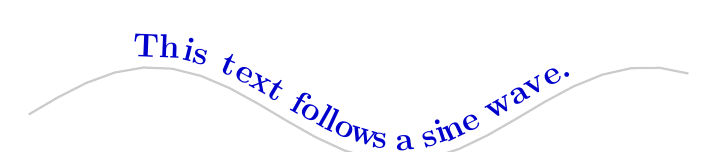
\begin{tikzpicture}
  \path [decorate, decoration={
    text along path,
    text={|\large\bfseries\color{blue!80!black}|~ This text follows a sine wave. ~},
    text align=center, raise=4pt
  }] plot[domain=0:8*pi/3, samples=24] (\x, {0.6*sin(deg(\x))});
  \draw[gray!40, thick] plot[domain=0:8*pi/3, samples=24] (\x, {0.6*sin(deg(\x))});
\end{tikzpicture}
\end{center}

\begin{center}
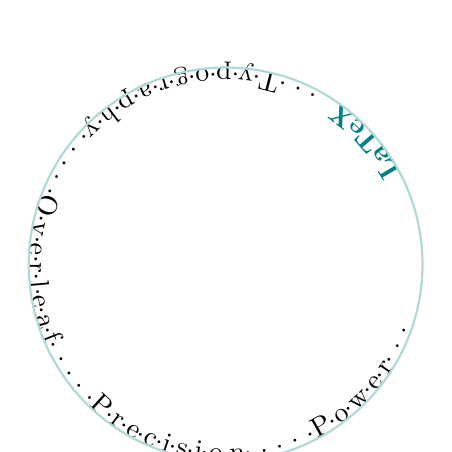
\begin{tikzpicture}
  \def\radius{2.5cm}
  \path [decorate, decoration={
    text along path,
    text={|\bfseries\color{teal}|~ LaTeX ~|$\cdot$|~ Typography ~|$\cdot$|~ Overleaf ~|$\cdot$|~ Precision ~|$\cdot$|~ Power ~|$\cdot$|},
    text align=center
  }] (0,0) circle (\radius);
  \draw[teal!30, thick] (0,0) circle (\radius);
\end{tikzpicture}
\end{center}

% ==============================================================
\section{Drop-Shadow Text (Pure TikZ)}
% ==============================================================

No external package needed --- a simple TikZ trick creates drop shadows on any text:

\begin{center}
\shadowtext{\Huge\bfseries\color{blue!70!black} Drop Shadow Text in \LaTeX}

\vspace{0.5cm}


\begin{tikzpicture}[baseline=(t.base)]
  \foreach \i in {4,3,2,1} {
    \node[opacity={0.06*\i}, yshift={-\i*0.8pt}, xshift={\i*0.8pt},
          text=black] at (0,0) {\Large\bfseries Multi-Layer Shadow Effect};
  }
  \node (t) [text=red!70!black] at (0,0) {\Large\bfseries Multi-Layer Shadow Effect};
\end{tikzpicture}
\end{center}

% ==============================================================
\section{Outlined / Stroked Text (\texttt{pdfrender})}
% ==============================================================

The old trick of drawing a box around a node only outlines the \emph{rectangle}.
\texttt{pdfrender} switches the PDF text-rendering mode itself, so the glyphs get a true
stroke around a separate fill:

\begin{center}
\vspace{0.3cm}
\textpdfrender{TextRenderingMode=FillStroke, FillColor=white, StrokeColor=blue!80!black,
  LineWidth=1.2pt}{\fontsize{44}{50}\selectfont\bfseries OUTLINE}
\quad
\textpdfrender{TextRenderingMode=FillStroke, FillColor=yellow, StrokeColor=red!70!black,
  LineWidth=0.8pt}{\fontsize{44}{50}\selectfont\bfseries GLOW}
\vspace{0.3cm}
\end{center}

% ==============================================================
\section{Absolute Positioning (\texttt{textpos})}
% ==============================================================

\begin{textblock}{5.5}(12.5, 21.0)
\begin{tcolorbox}[colback=orange!10, colframe=orange!80!black,
  title=\small Absolute Placement!, fonttitle=\bfseries\small,
  arc=3pt, boxrule=0.7pt]
\footnotesize This entire box is placed at coordinates (12.5\,cm, 21\,cm)
from the top-left corner of the page, completely ignoring normal text flow.
\end{tcolorbox}
\end{textblock}

This section demonstrates absolute coordinate positioning. The orange box floating
on this page is \textbf{not} part of the normal document flow --- it sits at an
absolute position on the physical page. Margin notes\marginnote{\footnotesize
\textcolor{purple}{\textbf{Margin note!}\\Parallel to the text it annotates.}}
work similarly, pinned to the current paragraph.

% ==============================================================
\section{Text in Geometric Shapes (\texttt{shapepar})}
% ==============================================================

\begin{center}
\heartpar{\color{red!70!black}\small
  In the beginning was the Word, and the Word was with \LaTeX.
  And suddenly all formatting nightmares ceased forever, for the
  compiler took dominion over rivers of white space and the scourge
  of the floating image that breaks the page. And it was good.
  Margins were aligned. References were automatically numbered.
  Tables did not break across sections. The bibliography was
  formatted unto perfection across every citation style known
  to academia. Chapters were stitched together from separate files.
  Equations were typeset with machine precision. The end.
}
\end{center}

\begin{center}
\diamondpar{\small
  This entire paragraph is constrained to flow inside a perfect
  diamond polygon computed entirely at compile time. No word processor
  can do this without inserting a pre-rendered image file. LaTeX
  computes the exact line widths needed at every vertical slice of
  the diamond and typesets each line to fit precisely, including
  proper automatic hyphenation at every break point. This is an
  extraordinary level of typographic control built directly into
  the language itself --- available to every LaTeX document, free.
}
\end{center}

% ==============================================================
\section{Dynamic Multiple Columns (\texttt{multicol})}
% ==============================================================

Unlike Word, \LaTeX{} can switch column layouts in the \emph{middle of a page} seamlessly:

\begin{multicols}{3}[\small\itshape Three balanced newspaper-style columns, mid-document:]
\noindent\lipsum[1][1-4]
\columnbreak
\noindent\lipsum[2][1-4]
\columnbreak
\noindent\lipsum[3][1-4]
\end{multicols}

% ==============================================================
\section{Relative Font Scaling (\texttt{relsize})}
% ==============================================================

\texttt{relsize} scales text \textit{relative} to the current font size, so it adapts
automatically even if you change the base font size later:

\bigskip
\begin{center}
{\relsize{-3} Tiny} \quad
{\relsize{-2} Smaller} \quad
{\relsize{-1} Small} \quad
{\relsize{0} Normal} \quad
{\relsize{1} Large} \quad
{\relsize{2} Larger} \quad
{\relsize{3} \textbf{Huge!}} \quad
{\relsize{4} \bfseries\color{blue!80!black} GIANT}
\end{center}

% ==============================================================
\section{Dingbats \& Symbol Fonts (\texttt{pifont})}
% ==============================================================

\newcommand{\cmark}{\ding{51}}
\newcommand{\xmark}{\ding{55}}
\newcommand{\starbullet}{\ding{72}}

\begin{center}
\begin{tabular}{lll}
\textcolor{green!60!black}{\cmark} Task complete &
\textcolor{red!70!black}{\xmark} Task failed &
\textcolor{orange!80!black}{\starbullet} Featured \\[4pt]
\ding{42} Pointing finger &
\ding{108} Filled circle &
\ding{167} Card suit \\[4pt]
\multicolumn{3}{c}{\ding{73}\ding{73}\ding{73}\ding{73} Rating: 4 stars \ding{73}\ding{73}\ding{73}\ding{73}} \\
\end{tabular}
\end{center}

\bigskip
Custom dingbat list bullets:
\begin{itemize}
  \renewcommand\labelitemi{\textcolor{blue}{\ding{117}}}
  \renewcommand\labelitemii{\textcolor{teal}{\ding{228}}}
  \item First item with a diamond bullet
  \item Second item
  \begin{itemize}
    \item Nested with an arrow bullet
    \item Another nested item
  \end{itemize}
\end{itemize}

% ==============================================================
\section{Inline Transformations (\texttt{graphicx})}
% ==============================================================

\texttt{graphicx} applies arbitrary affine transforms to \emph{any} content:

\bigskip
\noindent
\rotatebox{45}{\textbf{45{$^\circ$} rotation}} \quad
\rotatebox{-30}{\textcolor{red!70!black}{\textbf{$-30{^\circ}$ tilt}}} \quad
\scalebox{2.5}{\textbf{2.5$\times$}} \quad
\scalebox{1}[-1]{\textbf{Flipped vertically}} \quad
\reflectbox{\textbf{Mirror}} \quad
\resizebox{3cm}{!}{\textbf{Exactly 3\,cm wide}}

% ==============================================================
\section{tcolorbox --- Far Beyond Simple Boxes}
% ==============================================================

\begin{tcolorbox}[
  enhanced, arc=6pt,
  colback=blue!5!white, colframe=blue!75!black,
  title=\textbf{Standard Styled Box},
  attach boxed title to top center={yshift=-3mm},
  boxed title style={colback=blue!75!black, arc=4pt}
]
A basic \texttt{tcolorbox} already looks far more professional than anything
Word can produce natively without inserting a pre-made image.
\end{tcolorbox}

\vspace{0.5em}

\begin{tcolorbox}[
  enhanced,
  interior style={left color=red!20, right color=blue!20},
  frame style={left color=red!60!black, right color=blue!60!black},
  arc=8pt, boxrule=1.5pt,
  title=\textbf{\color{white}Gradient Interior Box}, fonttitle=\bfseries,
  attach boxed title to top left={yshift=-2.5mm, xshift=6mm},
  boxed title style={interior style={left color=red!60!black, right color=blue!60!black},
    arc=3pt, boxrule=0pt}
]
The interior and the frame both have \textbf{independent gradient fills}, specified
in pure \LaTeX{} code --- no image editor required.
\end{tcolorbox}

\vspace{0.5em}

\begin{tcolorbox}[
  enhanced, arc=0pt,
  colback=gray!5, colframe=gray!80,
  underlay={\begin{tcbclipinterior}
    \fill[red!20] (frame.south west) rectangle (frame.north west |- interior.south);
  \end{tcbclipinterior}},
  title=\textbf{Sidebar Accent Box}, fonttitle=\bfseries,
  left=8mm
]
This box has a coloured left-sidebar accent strip --- a design pattern common in
modern academic slides and technical documentation. Pure code, zero images.
\end{tcolorbox}

% ==============================================================
\section{TikZ Path Decorations (Wavy, Coil, Zigzag)}
% ==============================================================

\begin{center}

\begin{tikzpicture}
  \path [decorate, decoration={
      text along path,
      text={|\bfseries\color{purple}|~ Zigzag Path Typography in LaTeX ~},
      text align=center, raise=3pt
  }] (0,0) -- (1.5,0.7) -- (3,0) -- (4.5,0.7) -- (6,0) -- (7.5,0.7) -- (9,0);
  \draw[purple!30, thick, decorate, decoration=zigzag]
    (0,0) -- (9,0);
\end{tikzpicture}

\vspace{0.7cm}


\begin{tikzpicture}
  \draw[
    teal, line width=2pt,
    decorate, decoration={coil, amplitude=4pt, segment length=10pt}
  ] (0,0) -- (8,0)
    node[midway, above=10pt, teal, font=\small\bfseries]
      {Decorations: coils, snakes, bumps, zigzags, random steps\ldots};
\end{tikzpicture}
\end{center}

% ==============================================================
\section{Multi-Layer Letterpress / Emboss Effect (TikZ)}
% ==============================================================

\begin{center}
\vspace{0.5cm}

\begin{tikzpicture}
  \node[inner xsep=10pt, inner ysep=6pt, fill=black!85, rounded corners=4pt] (box) at (0,0) {
    \color{white}\Large\bfseries\tracked{PRECISION TYPOGRAPHY}
  };
  \node[inner sep=4pt, draw=yellow!80, line width=1pt,
        rounded corners=5pt, fit=(box)] {};
\end{tikzpicture}

\vspace{0.5cm}


\begin{tikzpicture}
  \node[text=gray!35] at (0.07, -0.07)
    {\fontsize{40}{50}\selectfont\bfseries \LaTeX};
  \node[text=gray!55] at (0.035, -0.035)
    {\fontsize{40}{50}\selectfont\bfseries \LaTeX};
  \node[text=blue!70!black] at (0,0)
    {\fontsize{40}{50}\selectfont\bfseries \LaTeX};
\end{tikzpicture}
\end{center}

% ==============================================================
\section{Niche Footnote Control (\texttt{footmisc})}
% ==============================================================

\texttt{footmisc} lets you change footnote markers to symbols\footnote{This is footnote one.}
instead of numbers, place footnotes in multiple columns, or prevent footnotes from splitting
across pages\footnote{This is footnote two --- notice the symbol markers (\dag, \ddag, etc.)
instead of numbers.} --- something Word handles very inconsistently.

% ==============================================================
\section{Custom Column Types and Zebra Tables (\texttt{array} + \texttt{colortbl})}
% ==============================================================

\texttt{array} lets you define reusable custom column types. Defined once, they work
everywhere in the document, and \verb|\rowcolors| stripes any table automatically:

\bigskip
\newcolumntype{C}[1]{>{\centering\arraybackslash\bfseries}m{#1}}
\newcolumntype{R}[1]{>{\raggedleft\arraybackslash\color{blue!70!black}}m{#1}}

\begin{center}
\renewcommand{\arraystretch}{1.6}
\begin{tabular}{C{3cm} R{3cm} >{\columncolor{green!10}}m{3.6cm}}
\toprule
\normalfont\textbf{Bold Center} &
\normalcolor\textbf{Colored Right} &
\textbf{Highlighted Column} \\
\midrule
Alpha   & 1,024   & \ding{51} Passed \\
Beta    & 48,992  & \ding{51} Passed \\
Gamma   & 3,141   & \ding{55} Failed \\
\bottomrule
\end{tabular}
\end{center}

\begin{center}
\rowcolors{2}{blue!8}{white}
\renewcommand{\arraystretch}{1.3}
\begin{tabular}{@{}lrrr@{}}
\rowcolor{blue!70!black}\color{white}\bfseries Package & \color{white}\bfseries Lines & \color{white}\bfseries Year & \color{white}\bfseries Used for \\
\texttt{tikz}      & 11k & 2005 & Graphics \\
\texttt{tcolorbox} & 14k & 2009 & Boxes \\
\texttt{pgfplots}  & 30k & 2007 & Plots \\
\texttt{microtype} & 9k  & 2004 & Spacing \\
\end{tabular}
\end{center}
{\footnotesize Sizes are rough, for illustration only.}

% ==============================================================
\section{Publication-Grade Mathematics (\texttt{amsmath}, \texttt{mathtools})}
% ==============================================================
% DESIGN: equations are semantic (\dd, \abs) so changing a convention is one line;
% tcolorbox adds highlighting and auto-numbered theorem boxes with no extra packages.

A displayed equation can be framed with \verb|\tcbhighmath|, and macros such as
\verb|\dd| keep the upright differential consistent everywhere:
\[ \tcbhighmath[colback=yellow!15, colframe=orange!70!black, boxrule=0.8pt, arc=3pt]{%
   e^{i\pi} + 1 = 0 } \]

\begin{align}
  \int_{-\infty}^{\infty} e^{-x^{2}} \dd x &= \sqrt{\pi}, &
  \sum_{n=1}^{\infty} \frac{1}{n^{2}} &= \frac{\pi^{2}}{6}, \\
  \zeta(s) &= \sum_{n=1}^{\infty} \frac{1}{n^{s}} = \prod_{p\ \text{prime}} \frac{1}{1-p^{-s}}, &
  \hat f(\xi) &= \int_{\mathbb{R}} f(x)\, e^{-2\pi i x\xi} \dd x.
\end{align}

Maxwell's equations, aligned on the relation symbols, and a piecewise function:
\begin{align*}
  \nabla\cdot\mathbf{E} &= \frac{\rho}{\varepsilon_0}, &
  \nabla\times\mathbf{E} &= -\frac{\partial\mathbf{B}}{\partial t}, \\
  \nabla\cdot\mathbf{B} &= 0, &
  \nabla\times\mathbf{B} &= \mu_0\!\left(\mathbf{J} + \varepsilon_0\frac{\partial\mathbf{E}}{\partial t}\right).
\end{align*}
\[
  R(\theta)=\begin{pmatrix}\cos\theta & -\sin\theta\\ \sin\theta & \cos\theta\end{pmatrix},
  \qquad
  \abs{x} = \begin{cases} x & x \ge 0,\\ -x & x < 0. \end{cases}
\]

\begin{thm}{Euclid}{euclid}
There are infinitely many prime numbers.
\end{thm}
\begin{proof}
Suppose $p_1,\dots,p_n$ were all the primes and let $N=p_1p_2\cdots p_n+1$. Dividing $N$ by
any $p_i$ leaves remainder $1$, so every prime factor of $N$ is missing from the list.
\end{proof}

% ==============================================================
\section{Data Visualisation (\texttt{pgfplots})}
% ==============================================================
% DESIGN: plots are drawn from formulas / coordinate lists at compile time, so fonts and
% colours match the document. Low sample counts keep the compile fast.

\begin{center}
\begin{minipage}[t]{0.48\textwidth}
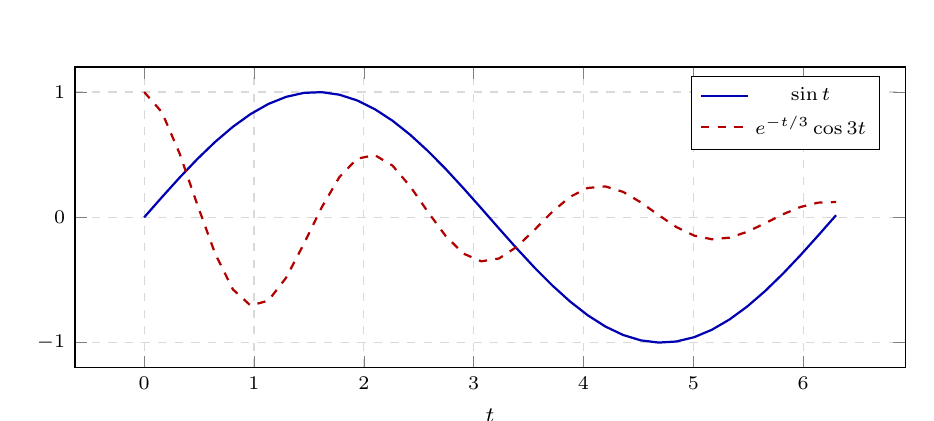
\begin{tikzpicture}
\begin{axis}[width=\linewidth, height=5.4cm, domain=0:6.3, samples=40, grid=major,
  grid style={dashed, gray!30}, xlabel={$t$}, legend pos=north east]
\addplot[thick, blue!70!black]{sin(deg(x))};
\addplot[thick, red!70!black, dashed]{exp(-x/3)*cos(deg(3*x))};
\legend{$\sin t$, $e^{-t/3}\cos 3t$}
\end{axis}
\end{tikzpicture}
\end{minipage}\hfill
\begin{minipage}[t]{0.48\textwidth}
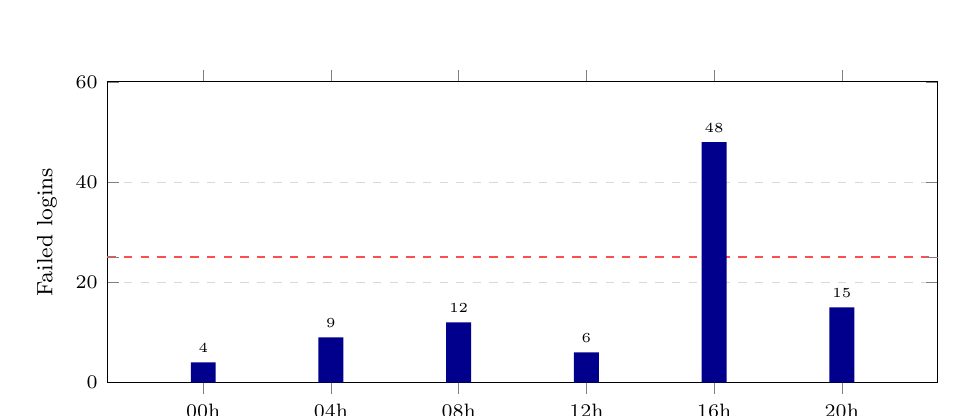
\begin{tikzpicture}
\begin{axis}[ybar, width=\linewidth, height=5.4cm, ymin=0, ymax=60,
  symbolic x coords={00h,04h,08h,12h,16h,20h}, xtick=data, bar width=9pt,
  enlarge x limits=0.15, ylabel={Failed logins}, ymajorgrids, grid style={dashed, gray!30},
  nodes near coords, nodes near coords style={font=\tiny},
  extra y ticks={25}, extra y tick labels={},
  extra y tick style={grid=major, grid style={red!70, dashed, thick}}]
\addplot[fill=blue!55!black, draw=none] coordinates
  {(00h,4) (04h,9) (08h,12) (12h,6) (16h,48) (20h,15)};
\end{axis}
\end{tikzpicture}
\end{minipage}
\end{center}
{\footnotesize Left: two functions from formulas. Right: illustrative data; the red line marks
an alert threshold.}

% ==============================================================
\section{Syntax-Highlighted Code (\texttt{listings} + \texttt{tcolorbox})}
% ==============================================================
% DESIGN: a listing style is defined once in the preamble; each box only names it,
% so every snippet in the document looks identical.

\begin{tcblisting}{listing only, enhanced, colback=gray!4, colframe=gray!60, arc=3pt,
  boxrule=0.5pt, title=\texttt{detector.py}, fonttitle=\small\bfseries,
  listing options={style=pycode}}
from collections import defaultdict, deque
import time

WINDOW, THRESHOLD = 60, 5            # seconds, failed attempts
attempts = defaultdict(deque)

def record_failure(ip, now=None):
    """Return True when `ip` should be blocked."""
    now = now or time.time()
    q = attempts[ip]
    q.append(now)
    while q and now - q[0] > WINDOW:  # drop stale events
        q.popleft()
    return len(q) >= THRESHOLD
\end{tcblisting}

% ==============================================================
\section{Diagrams as Code: Pipelines and Venn Sets (TikZ)}
% ==============================================================
% DESIGN: nodes are placed relative to each other (positioning library), so adding a
% stage never needs coordinates to be recalculated; \texttt{fit} draws the group frame.

\begin{center}
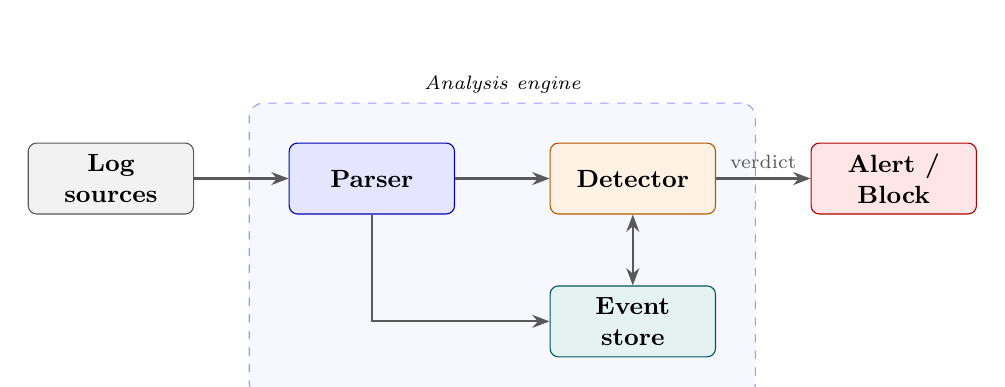
\begin{tikzpicture}[node distance=9mm and 12mm, >={Stealth[length=2.2mm]},
  box/.style={draw=#1!70!black, fill=#1!10, rounded corners=3pt, minimum height=9mm,
    minimum width=21mm, align=center, font=\small\bfseries},
  flow/.style={->, thick, gray!70!black}]
  \node[box=gray]   (src)   {Log\\sources};
  \node[box=blue,   right=of src]   (parse) {Parser};
  \node[box=orange, right=of parse] (det)   {Detector};
  \node[box=red,    right=of det]   (act)   {Alert /\\Block};
  \node[box=teal,   below=of det]   (store) {Event\\store};
  \draw[flow] (src) -- (parse);
  \draw[flow] (parse) -- (det);
  \draw[flow] (det) -- (act) node[midway, above, font=\scriptsize] {verdict};
  \draw[flow] (parse) |- (store);
  \draw[flow, <->] (det) -- (store);
  \begin{scope}[on background layer]
    \node[draw=blue!40, dashed, rounded corners=5pt, fill=blue!3, inner sep=5mm,
      fit=(parse)(det)(store), label={[font=\scriptsize\itshape]above:Analysis engine}] {};
  \end{scope}
\end{tikzpicture}
\end{center}

\begin{minipage}[c]{0.52\textwidth}
Sets overlap in a way no table can show. The security ``CIA triad'' is the classic
three-circle Venn diagram: a system is \emph{secure} only where all three goals meet.
Circle fills use \texttt{fill opacity}, so the overlaps mix colours automatically.
\end{minipage}\hfill
\begin{minipage}[c]{0.42\textwidth}
\centering
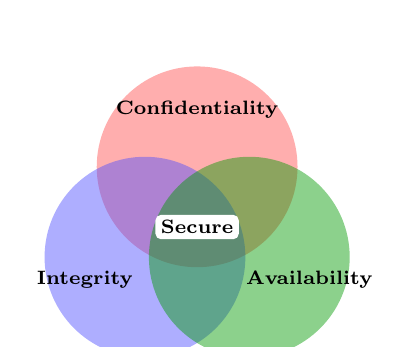
\begin{tikzpicture}[scale=0.85]
  \begin{scope}[fill opacity=0.45]
    \fill[red!70]            (90:0.9)  circle (1.5);
    \fill[blue!70]           (210:0.9) circle (1.5);
    \fill[green!60!black]    (330:0.9) circle (1.5);
  \end{scope}
  \node[font=\scriptsize\bfseries] at (90:1.75)  {Confidentiality};
  \node[font=\scriptsize\bfseries] at (205:1.85) {Integrity};
  \node[font=\scriptsize\bfseries] at (335:1.85) {Availability};
  \node[font=\scriptsize\bfseries, fill=white, rounded corners=2pt, inner sep=2pt] at (0,0) {Secure};
\end{tikzpicture}
\end{minipage}

% ==============================================================
\section{Protocol Diagrams (\texttt{bytefield})}
% ==============================================================
% DESIGN: the header is described field-by-field with its bit widths, so the drawing
% cannot drift out of sync with the specification.

\begin{center}
\begin{bytefield}[bitwidth=0.95em]{32}
  \bitheader{0,15,16,31} \\
  \bitbox{16}{Source Port} & \bitbox{16}{Destination Port} \\
  \bitbox{32}{Sequence Number} \\
  \bitbox{32}{Acknowledgment Number} \\
  \bitbox{4}{\tiny Offset} & \bitbox{6}{\tiny Reserved} &
  \bitbox{1}{\tiny U} & \bitbox{1}{\tiny A} & \bitbox{1}{\tiny P} &
  \bitbox{1}{\tiny R} & \bitbox{1}{\tiny S} & \bitbox{1}{\tiny F} &
  \bitbox{16}{Window Size} \\
  \bitbox{16}{Checksum} & \bitbox{16}{Urgent Pointer} \\
  \wordbox{1}{Options and padding (variable length)}
\end{bytefield}
\end{center}
\begin{center}\small\itshape A TCP header, drawn from its field widths.\end{center}

% ==============================================================
\section{Fractals from Rewriting Rules (TikZ)}
% ==============================================================
% DESIGN: each curve is a tiny grammar (axiom + rules) expanded at compile time; the
% order is capped at a level that still looks sharp but compiles in a fraction of a second.

\begin{center}
\begin{minipage}[b]{0.32\textwidth}\centering

\begin{tikzpicture}[scale=0.62]
  \draw[blue!70!black, thick] decorate[decoration=Koch snowflake]{decorate{decorate{
    (0,0) -- ++(60:4) -- ++(-60:4) -- cycle}}};
\end{tikzpicture}\\[2pt]\small Koch snowflake
\end{minipage}\hfill
\begin{minipage}[b]{0.32\textwidth}\centering
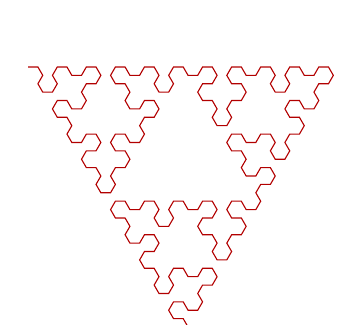
\begin{tikzpicture}
  \draw[red!70!black, line width=0.4pt] lindenmayer system
    [l-system={Sierpinski, axiom=X, order=5, step=3.5pt, angle=60}];
\end{tikzpicture}\\[2pt]\small Sierpinski triangle
\end{minipage}\hfill
\begin{minipage}[b]{0.32\textwidth}\centering
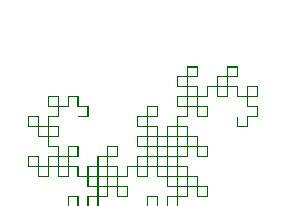
\begin{tikzpicture}
  \draw[green!40!black, line width=0.4pt] lindenmayer system
    [l-system={Dragon, axiom=FX, order=8, step=3.6pt, angle=90}];
\end{tikzpicture}\\[2pt]\small Dragon curve
\end{minipage}
\end{center}

% ==============================================================
\newpage
\section{Mastering Images: Placement, Clipping, and Wrapping}
% ==============================================================

While Word often struggles with image placement (the infamous ``move an image 1mm and ruin the document''), \LaTeX{} provides absolute, predictable control. Here are the most powerful ways to handle images natively.

\subsection*{1. Text Wrapping (\texttt{wrapfig})}
The \texttt{wrapfigure} environment lets text flow naturally around an image.
\begin{wrapfigure}{r}{0.35\textwidth}
  \vspace{-15pt}
  \centering
  \includegraphics[width=\linewidth]{example-image-a}
  \caption{Wrapped Image}
  \vspace{-10pt}
\end{wrapfigure}
\lipsum[1][1-5] This text continues to wrap around the image on the right side of the page, demonstrating how \LaTeX{} automatically adjusts the paragraph margins to accommodate floating elements seamlessly without breaking the flow.

\subsection*{2. Side-by-Side Subfigures (\texttt{subcaption})}
When you need multiple related images aligned perfectly, \texttt{subfigure} handles it flawlessly:

\begin{figure}[H]
  \centering
  \begin{subfigure}[b]{0.45\textwidth}
    \centering
    \includegraphics[width=\textwidth]{example-image-b}
    \caption{First side-by-side image}
  \end{subfigure}
  \hfill
  \begin{subfigure}[b]{0.45\textwidth}
    \centering
    \includegraphics[width=\textwidth]{example-image-c}
    \caption{Second side-by-side image}
  \end{subfigure}
  \caption{A perfectly aligned dual-image setup.}
\end{figure}

\subsection*{3. Forcing Absolute Placement (\texttt{float})}
If you ever want an image to appear \textbf{exactly here} without floating to the top of the next page, use the \texttt{[H]} specifier provided by the \texttt{float} package:

\begin{figure}[H]
  \centering
  \includegraphics[width=4cm]{example-image}
  \caption{This image will not float. It is anchored \texttt{[H]}ere.}
\end{figure}

\subsection*{4. Arbitrary Clipping and Shapes (TikZ)}
Instead of cropping images in an external editor, you can clip them directly in \LaTeX{} using TikZ. Here we clip a standard rectangular image into a perfect circle:

\begin{center}

\begin{tikzpicture}
  \clip (0,0) circle (2.2cm);
  \node at (0,0) {\includegraphics[width=6cm]{example-image-a}};
\end{tikzpicture}
\end{center}

\subsection*{5. Images inside Flowcharts (TikZ)}
You can integrate images directly into flowchart nodes, which suits architecture diagrams or process flows with embedded screenshots or photos.

\begin{center}
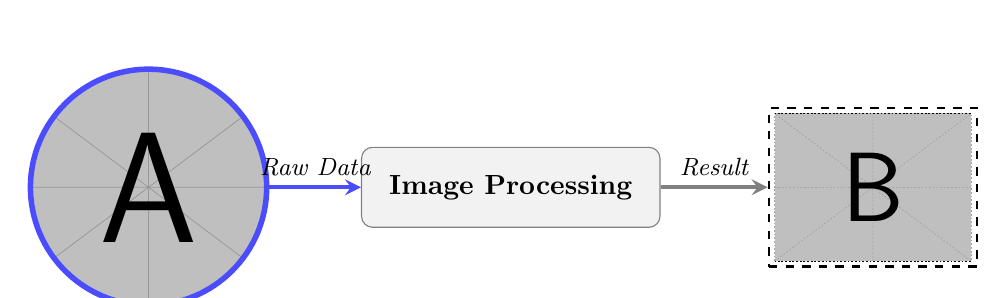
\begin{tikzpicture}[node distance=4.6cm]
  \node (input) [circle, draw=blue!70, line width=2pt, minimum size=3cm, path picture={
    \node at (path picture bounding box.center) {\includegraphics[height=3cm]{example-image-a}};
  }] {};
  \node (process) [right of=input, rectangle, draw=gray, fill=gray!10, rounded corners, inner sep=10pt, font=\bfseries] {Image Processing};
  \node (output) [right of=process, draw=black, dashed, line width=1pt, inner sep=2pt] {\includegraphics[width=2.5cm]{example-image-b}};
  \draw[->, >=stealth, line width=1.5pt, blue!70] (input) -- (process) node[midway, above, font=\small\itshape, text=black] {Raw Data};
  \draw[->, >=stealth, line width=1.5pt, gray] (process) -- (output) node[midway, above, font=\small\itshape, text=black] {Result};
\end{tikzpicture}
\end{center}

% ==============================================================
\newpage
\section{Pushing the Limits --- Niche Specialist Packages}
% ==============================================================

\begin{tcolorbox}[niche=purple, title={The Big Reveal}]
These are things virtually no one expects a text document to be able to produce from
\textbf{pure code}. Each one is a single \texttt{\textbackslash usepackage\{\}} declaration.
\end{tcolorbox}

% ------------------------------------------------------------------
\subsection*{Sheet Music (\texttt{musixtex})}
% ------------------------------------------------------------------
\texttt{musixtex} renders engraver-quality sheet music --- bar lines, note heads, stems,
time signatures, slurs, and dynamics --- all from code:

\begin{center}
\begin{music}
\parindent10mm
\instrumentnumber{1}
\setstaffs1{1}
\generalmeter{\meterfrac{4}{4}}
\startextract
\Notes \qu c \qu d \qu e \qu f \en
\Notes \ql g \ql h \ql i \qu j \en
\Notes \hu k \hu l \en
\endextract
\end{music}
\end{center}

% ------------------------------------------------------------------
\subsection*{Chemical Structures (\texttt{chemfig})}
% ------------------------------------------------------------------
\texttt{chemfig} draws 2D structural formulae from a compact bond-and-atom syntax:

\begin{center}
\renewcommand{\arraystretch}{1}
\begin{tabular}{ccc}
\chemfig{*6(-=-=-=)} & \chemfig{H_3C-C(=[1]O)-OH} & \chemfig{H_3C-CH_2-OH} \\[0.4cm]
\small Benzene & \small Acetic acid & \small Ethanol
\end{tabular}
\end{center}

% ------------------------------------------------------------------
\subsection*{Circuit Schematics (\texttt{circuitikz})}
% ------------------------------------------------------------------
\texttt{circuitikz} draws professional electronic circuit diagrams with proper IEEE/IEC symbols:

\begin{center}
\begin{circuitikz}[scale=0.85, transform shape]
  \draw (0,0)
    to[V, v=$V_s$, invert] (0,3)
    to[R, l=$R$] (3,3)
    to[C, l=$C$] (3,0)
    -- (0,0);
  \draw (3,3) to[short] (5,3)
    to[voltmeter, l=$V_C$] (5,0)
    to[short] (3,0);
  \draw (0,0) node[ground]{};
\end{circuitikz}
\end{center}

% ------------------------------------------------------------------
\subsection*{Chess Boards (\texttt{skak})}
% ------------------------------------------------------------------
\texttt{skak} renders full 8$\times$8 chessboards with proper piece glyphs. You feed it
standard algebraic notation and it computes the position:

\begin{center}
\newgame
\mainline{1.e4 e5 2.Nf3 Nc6 3.Bc4 Bc5 4.b4}
\showboard
\end{center}
\begin{center}
\small\textit{Position after 4.b4 --- The Evans Gambit, rendered 100\% in \LaTeX{}}
\end{center}

% ------------------------------------------------------------------
\subsection*{Crossword Puzzles (Pure TikZ)}
% ------------------------------------------------------------------
A crossword grid with numbered squares, drawn from a list of cells. The grid below is
consistent with its clues:

\begin{center}
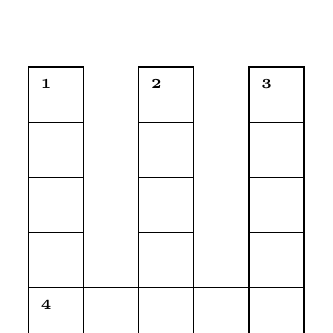
\begin{tikzpicture}[scale=0.7]
  \foreach \x/\y in {0/4,0/3,0/2,0/1,0/0, 2/4,2/3,2/2,2/1,2/0, 4/4,4/3,4/2,4/1,4/0, 1/0,3/0}
    \draw[fill=white, line width=0.5pt] (\x,\y) rectangle ++(1,1);
  \node[anchor=north west, font=\tiny\bfseries] at (0.05,4.95) {1};
  \node[anchor=north west, font=\tiny\bfseries] at (2.05,4.95) {2};
  \node[anchor=north west, font=\tiny\bfseries] at (4.05,4.95) {3};
  \node[anchor=north west, font=\tiny\bfseries] at (0.05,0.95) {4};
\end{tikzpicture}
\end{center}

\noindent
\begin{minipage}[t]{0.45\textwidth}
\textbf{Across:}\\[2pt]
\textbf{4.} The system you are reading right now (5)
\end{minipage}\hfill
\begin{minipage}[t]{0.45\textwidth}
\textbf{Down:}\\[2pt]
\textbf{1.} A tag you can attach to an equation (5)\\[1pt]
\textbf{2.} What a program reads from the keyboard (5)\\[1pt]
\textbf{3.} Open-source kernel with a penguin (5)
\end{minipage}

\medskip
\noindent{\footnotesize Solution (upside down): \rotatebox{180}{LABEL \ INPUT \ LINUX \ LATEX}}

% ------------------------------------------------------------------
\subsection*{Rubik's Cube Diagrams (Pure TikZ Isometric)}
% ------------------------------------------------------------------
A 3D isometric cube drawn with one reusable macro. The stickers on the left are a
pseudo-random pattern, the right cube is solved:

\begin{center}
\rubik{1}\hspace{1.5cm}\rubik{0}

{\small\itshape Scrambled (illustrative) \hspace{3.2cm} Solved}
\end{center}

% ------------------------------------------------------------------
\subsection*{QR Codes (\texttt{qrcode})}
% ------------------------------------------------------------------
\begin{minipage}[c]{0.2\textwidth}
\qrcode[height=2.4cm]{https://ctan.org}
\end{minipage}\hfill
\begin{minipage}[c]{0.74\textwidth}
This QR code is generated by \LaTeX{} itself, as vector graphics, with no image file.
It points to \url{https://ctan.org}, the archive that hosts the packages used here.
\end{minipage}

\bigskip
\begin{tcolorbox}[
  enhanced, arc=0pt,
  colback=gray!5, colframe=gray!80,
  underlay={\begin{tcbclipinterior}
    \fill[yellow!60!orange] (frame.south west) rectangle (frame.north west |- interior.south);
  \end{tcbclipinterior}},
  title=\textbf{The Cheat Code}, fonttitle=\bfseries,
  left=8mm
]
If you can \textbf{describe} something mathematically or structurally, \LaTeX{} can
\textbf{typeset} it. Search CTAN (\texttt{ctan.org}) for any niche domain. The question is
never \textit{can \LaTeX{} do this?} The question is only \textit{which package?}
\end{tcolorbox}

\end{document}
